% 2.2 Job Submission Basics
% -------------------------------------------------------------
\subsection{Job Submission Basics}
\label{sect:job-submission-basics}

Preparing your job for submission is fairly straightforward.
Start by basing your job script on one of the examples available in the \texttt{src/}
directory of our \href{https://github.com/NAG-DevOps/speed-hpc}{GitHub repository}.
You can clone the repository to get the examples to start with via the command line:

\begin{verbatim}
    git clone --depth=1 https://github.com/NAG-DevOps/speed-hpc.git
    cd speed-hpc/src
\end{verbatim}

\noindent The job script is a shell script that contains directives, module loads, and user scripting.
To quickly run some sample jobs, use the following commands:
\begin{verbatim}
    sbatch -p ps -t 10 env.sh
    sbatch -p ps -t 10 bash.sh
    sbatch -p ps -t 10 manual.sh
    sbatch -p pg -t 10 lambdal-singularity.sh
\end{verbatim}

%  2.2.1 Directives
% -------------------
\subsubsection{Directives}
\label{sect:directives}
% ------------------------------------------------------------------------------
\subsubsection{Directives}
\label{sect:directives}

Directives are comments included at the beginning of a job script that set the shell 
and the options for the job scheduler. 
%
The shebang directive is always the first line of a script. In your job script, 
this directive sets which shell your script's commands will run in. On ``Speed'', 
we recommend that your script use a shell from the \texttt{/encs/bin} directory. 

To use the \texttt{tcsh} shell, start your script with \verb|#!/encs/bin/tcsh|.
%
For \texttt{bash}, start with \verb|#!/encs/bin/bash|.
%
Directives that start with \verb|#SBATCH|, set the options for the cluster's 
Slurm job scheduler. The script template, \texttt{template.sh}, 
provides the essentials:

%\begin{verbatim}
%#$ -N <jobname>
%#$ -cwd
%#$ -m bea
%#$ -pe smp <corecount>
%#$ -l h_vmem=<memory>G
%\end{verbatim}
\begin{verbatim}
#SBATCH --job-name=<jobname>        ## or -J. Give the job a name 
#SBATCH --mail-type=<type>          ## Set type of email notifications
#SBATCH --chdir=<directory>         ## or -D, Set working directory where output files will go 
#SBATCH --nodes=1                   ## or -N, Node count required for the job
#SBATCH --ntasks=1                  ## or -n, Number of tasks to be launched
#SBATCH --cpus-per-task=<corecount> ## or -c, Core count requested, e.g. 8 cores
#SBATCH --mem=<memory>              ## Assign memory for this job, e.g., 32G memory per node 
\end{verbatim}

Replace the following to adjust the job script for your project(s)
\begin{enumerate}
  \item \verb+<jobname>+ with a job name for the job
  \item \verb+<directory>+ with the fullpath to your job's working directory, e.g., where your code,
source files and where the standard output files will be written to. By default, \verb+--chdir+
sets the current directory as the job's working directory 
  \item \verb+<type>+ with the type of e-mail notifications you wish to receive. Valid options are: NONE, BEGIN, END, FAIL, REQUEUE, ALL 
  \item \verb+<corecount>+ with the degree of multithreaded parallelism (i.e., cores) allocated to your job. Up to 32 by default.
  \item \verb+<memory>+ with the amount of memory, in GB, that you want to be allocated per node. Up to 500 depending on the node. 
  NOTE: All jobs MUST set a value for the \verb|--mem| option.
\end{enumerate}

Example with short option equivalents:

\begin{verbatim}
#SBATCH -J tmpdir                   ## Job's name set to 'tmpdir'
#SBATCH --mail-type=ALL             ## Receive all email type notifications
#SBATCH -D ./                       ## Use current directory as working directory
#SBATCH -N 1                        ## Node count required for the job
#SBATCH -n 1                        ## Number of tasks to be launched
#SBATCH -c 8                        ## Request 8 cores
#SBATCH --mem=32G                   ## Allocate 32G memory per node 
\end{verbatim}

%
If you are unsure about memory footprints, err on assigning a generous
memory space to your job, so that it does not get prematurely terminated.
%(the value given to \api{h\_vmem} is a hard memory ceiling).
You can refine
%\api{h\_vmem}
\option{--mem}
values for future jobs by monitoring the size of a job's active
memory space on \texttt{speed-submit} with:

%\begin{verbatim}
%qstat -j <jobID> | grep maxvmem
%\end{verbatim}

\begin{verbatim}
sacct -j <jobID>
sstat -j <jobID>
\end{verbatim}

\noindent
This can be customized to show specific columns:

\begin{verbatim}
sacct -o jobid,maxvmsize,ntasks%7,tresusageouttot%25 -j <jobID>
sstat -o jobid,maxvmsize,ntasks%7,tresusageouttot%25 -j <jobID>
\end{verbatim}

Memory-footprint values are also provided for completed jobs in the final
e-mail notification as ``maxvmsize''.
%
\emph{Jobs that request a low-memory footprint are more likely to load on a busy
cluster.}

Other essential options are \option{--time}, or \verb|-t|, and \option{--account}, or \verb|-A|.
%
\begin{itemize}
\item
\option{--time=<time>} -- is the estimate of wall clock time required for your job to run. 
As preiviously mentioned, the maximum is 7 days for batch and 24 hours for interactive jobs. 
Jobs with a smaller \texttt{time} value will have a higher priority and may result in your job being scheduled sooner. 

\item
\option{--account=<name>} -- specifies which Account, aka project or association, 
that the Speed resources your job uses should be attributed to. When moving from 
GE to SLURM users most users were assigned to Speed's two default accounts 
\texttt{speed1} and \texttt{speed2}. However, users that belong to a particular research
group or project are will have a default Account like the following
\texttt{aits},
\texttt{vidpro},
\texttt{gipsy},
\texttt{ai2},
\texttt{mpackir},
\texttt{cmos}, among others.

\end{itemize}
%TO BE DELETED
%% ------------------------------------------------------------------------------
\subsubsection{Directives}
\label{sect:directives}

Directives are comments included at the beginning of a job script that set the shell 
and the options for the job scheduler. 
%
The shebang directive is always the first line of a script. In your job script, 
this directive sets which shell your script's commands will run in. On ``Speed'', 
we recommend that your script use a shell from the \texttt{/encs/bin} directory. 

To use the \texttt{tcsh} shell, start your script with \verb|#!/encs/bin/tcsh|.
%
For \texttt{bash}, start with \verb|#!/encs/bin/bash|.
%
Directives that start with \verb|#SBATCH|, set the options for the cluster's 
Slurm job scheduler. The script template, \texttt{template.sh}, 
provides the essentials:

%\begin{verbatim}
%#$ -N <jobname>
%#$ -cwd
%#$ -m bea
%#$ -pe smp <corecount>
%#$ -l h_vmem=<memory>G
%\end{verbatim}
\begin{verbatim}
#SBATCH --job-name=<jobname>        ## or -J. Give the job a name 
#SBATCH --mail-type=<type>          ## Set type of email notifications
#SBATCH --chdir=<directory>         ## or -D, Set working directory where output files will go 
#SBATCH --nodes=1                   ## or -N, Node count required for the job
#SBATCH --ntasks=1                  ## or -n, Number of tasks to be launched
#SBATCH --cpus-per-task=<corecount> ## or -c, Core count requested, e.g. 8 cores
#SBATCH --mem=<memory>              ## Assign memory for this job, e.g., 32G memory per node 
\end{verbatim}

Replace the following to adjust the job script for your project(s)
\begin{enumerate}
  \item \verb+<jobname>+ with a job name for the job
  \item \verb+<directory>+ with the fullpath to your job's working directory, e.g., where your code,
source files and where the standard output files will be written to. By default, \verb+--chdir+
sets the current directory as the job's working directory 
  \item \verb+<type>+ with the type of e-mail notifications you wish to receive. Valid options are: NONE, BEGIN, END, FAIL, REQUEUE, ALL 
  \item \verb+<corecount>+ with the degree of multithreaded parallelism (i.e., cores) allocated to your job. Up to 32 by default.
  \item \verb+<memory>+ with the amount of memory, in GB, that you want to be allocated per node. Up to 500 depending on the node. 
  NOTE: All jobs MUST set a value for the \verb|--mem| option.
\end{enumerate}

Example with short option equivalents:

\begin{verbatim}
#SBATCH -J tmpdir                   ## Job's name set to 'tmpdir'
#SBATCH --mail-type=ALL             ## Receive all email type notifications
#SBATCH -D ./                       ## Use current directory as working directory
#SBATCH -N 1                        ## Node count required for the job
#SBATCH -n 1                        ## Number of tasks to be launched
#SBATCH -c 8                        ## Request 8 cores
#SBATCH --mem=32G                   ## Allocate 32G memory per node 
\end{verbatim}

%
If you are unsure about memory footprints, err on assigning a generous
memory space to your job, so that it does not get prematurely terminated.
%(the value given to \api{h\_vmem} is a hard memory ceiling).
You can refine
%\api{h\_vmem}
\option{--mem}
values for future jobs by monitoring the size of a job's active
memory space on \texttt{speed-submit} with:

%\begin{verbatim}
%qstat -j <jobID> | grep maxvmem
%\end{verbatim}

\begin{verbatim}
sacct -j <jobID>
sstat -j <jobID>
\end{verbatim}

\noindent
This can be customized to show specific columns:

\begin{verbatim}
sacct -o jobid,maxvmsize,ntasks%7,tresusageouttot%25 -j <jobID>
sstat -o jobid,maxvmsize,ntasks%7,tresusageouttot%25 -j <jobID>
\end{verbatim}

Memory-footprint values are also provided for completed jobs in the final
e-mail notification as ``maxvmsize''.
%
\emph{Jobs that request a low-memory footprint are more likely to load on a busy
cluster.}

Other essential options are \option{--time}, or \verb|-t|, and \option{--account}, or \verb|-A|.
%
\begin{itemize}
\item
\option{--time=<time>} -- is the estimate of wall clock time required for your job to run. 
As preiviously mentioned, the maximum is 7 days for batch and 24 hours for interactive jobs. 
Jobs with a smaller \texttt{time} value will have a higher priority and may result in your job being scheduled sooner. 

\item
\option{--account=<name>} -- specifies which Account, aka project or association, 
that the Speed resources your job uses should be attributed to. When moving from 
GE to SLURM users most users were assigned to Speed's two default accounts 
\texttt{speed1} and \texttt{speed2}. However, users that belong to a particular research
group or project are will have a default Account like the following
\texttt{aits},
\texttt{vidpro},
\texttt{gipsy},
\texttt{ai2},
\texttt{mpackir},
\texttt{cmos}, among others.

\end{itemize}
%

Directives are comments included at the beginning of a job script that set the shell
and the options for the job scheduler.

The shebang directive is always the first line of a script. In your job script,
this directive sets which shell your script's commands will run in. On ``Speed'',
we recommend that your script use a shell from the \texttt{/encs/bin} directory.

To use \texttt{tcsh} shell, start your script with \verb|#!/encs/bin/tcsh|. For \texttt{bash}, use \verb|#!/encs/bin/bash| instead.

Directives that start with \verb|#SBATCH| set the options for the cluster's SLURM job scheduler.
The following provides an example of some essential directives:

\small
\begin{verbatim}
    #SBATCH --job-name=<jobname>        ## or -J. Give the job a name
    #SBATCH --mail-type=<type>          ## set type of email notifications
    #SBATCH --chdir=<directory>         ## or -D, set working directory for the job
    #SBATCH --nodes=1                   ## or -N, node count required for the job
    #SBATCH --ntasks=1                  ## or -n, number of tasks to be launched
    #SBATCH --cpus-per-task=<corecount> ## or -c, core count requested, e.g. 8 cores
    #SBATCH --mem=<memory>              ## assign memory for this job,
                                        ## e.g., 32G memory per node
\end{verbatim}
\normalsize

\noindent Replace the following to adjust the job script for your project(s)
\begin{itemize}
    \item \verb+<jobname>+ with a job name for the job. This name will be displayed in the job queue.
    \item \verb+<directory>+ with the fullpath to your job's working directory, e.g., where your code,
    source files and where the standard output files will be written to.
    By default, \verb+--chdir+ sets the current directory as the job's working directory.
    \item \verb+<type>+ with the type of e-mail notifications you wish to receive.
    Valid options are: NONE, BEGIN, END, FAIL, REQUEUE, ALL.
    \item \verb+<corecount>+ with the degree of multithreaded parallelism (i.e., cores) allocated to your job. Up to 32 by default.
    \item \verb+<memory>+ with the amount of memory, in GB, that you want to be allocated per node. Up to 500 depending on the node.\\
    \textbf{Note}: All jobs MUST set a value for the \option{--mem} option.
\end{itemize}

\noindent Example with short option equivalents:
\small
\begin{verbatim}
    #SBATCH -J myjob              ## Job's name set to 'myjob'
    #SBATCH --mail-type=ALL       ## Receive all email type notifications
    #SBATCH -D ./                 ## Use current directory as working directory
    #SBATCH -N 1                  ## Node count required for the job
    #SBATCH -n 1                  ## Number of tasks to be launched
    #SBATCH -c 8                  ## Request 8 cores
    #SBATCH --mem=32G             ## Allocate 32G memory per node
\end{verbatim}
\normalsize

\noindent \textbf{Tip:} If you are unsure about memory footprints, err on assigning a generous
memory space to your job, so that it does not get prematurely terminated.
You can refine \option{--mem} values for future jobs by monitoring the size of a job's active
memory space on \texttt{speed-submit} with:

\begin{verbatim}
    sacct -j <jobID>
    sstat -j <jobID>
\end{verbatim}

\noindent This can be customized to show specific columns:

\begin{verbatim}
    sacct -o jobid,maxvmsize,ntasks%7,tresusageouttot%25 -j <jobID>
    sstat -o jobid,maxvmsize,ntasks%7,tresusageouttot%25 -j <jobID>
\end{verbatim}

\noindent Memory-footprint efficiency values \tool{seff} are also provided for completed jobs
in the final email notification as ``maxvmsize''.

\emph{Jobs that request a low-memory footprint are more likely to load on a busy cluster.}

\noindent Other essential options are \option{--time}, or \option{-t}, and \option{--account}, or \option{-A}.
\begin{itemize}
    \item \option{--time=<time>} -- is the estimate of wall clock time required for your job to run.
    As previously mentioned, the maximum is 7 days for batch and 24 hours for interactive jobs.
    Jobs with a smaller \texttt{time} value will have a higher priority and may result in your job being scheduled sooner.
    \item \option{--account=<name>} -- specifies which Account, aka project or association,
    that the Speed resources your job uses should be attributed to. When moving from
    GE to SLURM users most users were assigned to Speed's two default accounts
    \texttt{speed1} and \texttt{speed2}. However, users that belong to a particular research
    group or project are will have a default Account like the following
    \texttt{aits},
    \texttt{vidpro},
    \texttt{gipsy},
    \texttt{ai2},
    \texttt{mpackir},
    \texttt{cmos}, among others.
\end{itemize}

%  2.2.2 Module Loads
% -------------------
\subsubsection{Working with Modules}
\label{sect:modules}

After setting the directives in your job script, the next section typically involves loading
the necessary software modules. The \tool{module} command is used to manage the user environment,
make sure to load all the modules your job depends on. You can check available modules with the
module avail command. Loading the correct modules ensures that your environment is properly
set up for execution.

\noindent To list for a particular program (\tool{matlab}, for example):
\small
\begin{verbatim}
    module avail
    module -t avail matlab  ## show the list for a particular program (e.g., matlab)
    module -t avail m       ## show the list for all programs starting with `m'
\end{verbatim}
\normalsize

For example, insert the following in your script to load the \tool{matlab/R2023a} module:
\begin{verbatim}
    module load matlab/R2023a/default
\end{verbatim}

\textbf{Note:} you can remove a module from active use by replacing \option{load} by \option{unload}.

To list loaded modules:
\begin{verbatim}
    module list
\end{verbatim}

To purge all software in your working environment:
\begin{verbatim}
    module purge
\end{verbatim}

%  2.2.3 User Scripting
% -------------------
\subsubsection{User Scripting}
\label{sect:scripting}
%TO BE DELETED
%% ------------------------------------------------------------------------------
\subsubsection{User Scripting}
\label{sect:scripting}

The last part the job script is the scripting that will be executed by the job. 
This part of the job script includes all commands required to set up and 
execute the task your script has been written to do. Any Linux command can be used 
at this step. This section can be a simple call to an executable or a complex 
loop which iterates through a series of commands.

Any compute heavy step is preferably should be prefixed by \tool{srun}
as the best practice.

Every software program has a unique execution framework. It is the responsibility 
of the script's author (e.g., you) to know what is required for the software used 
in your script by reviewing the software's documentation. Regardless of which software
your script calls, your script should be written so that the software knows the 
location of the input and output files as well as the degree of parallelism.
%
% GE:
%Note that the cluster-specific environment variable, \api{NSLOTS}, resolves 
%to the value provided to the scheduler in the \option{-pe smp} option. 

Jobs which touch data-input and data-output files more than once, should make use 
of \api{TMPDIR}, a scheduler-provided working space almost 1~TB in size.
\api{TMPDIR} is created when a job starts, and exists on the local disk of the
compute node executing your job. Using \api{TMPDIR} results in faster I/O operations 
than those to and from shared storage (which is provided over NFS). 

An sample job script using \api{TMPDIR} is available at \texttt{/home/n/nul-uge/templateTMPDIR.sh}: 
the job is instructed to change to \api{\$TMPDIR}, to make the new directory \texttt{input}, to copy data from
%\texttt{\$SGE\_O\_WORKDIR/references/} to \texttt{input/} (\texttt{\$SGE\_O\_WORKDIR} represents the
\texttt{\$SLURM\_SUBMIT\_DIR/references/} to \texttt{input/} (\texttt{\$SLURM\_SUBMIT\_DIR} represents the
current working directory), to make the new directory \texttt{results}, to
execute the program (which takes input from \texttt{\$TMPDIR/input/} and writes
output to \texttt{\$TMPDIR/results/}), and finally to copy the total end results
to an existing directory, \texttt{processed}, that is located in the current
working directory.
% TODO: verify:
TMPDIR only exists for the duration of the job, though,
so it is very important to copy relevant results from it at job's end.

% ------------------------------------------------------------------------------
\subsection{Sample Job Script}

Now, let's look at a basic job script, \file{tcsh.sh} in \xf{fig:tcsh.sh}
(you can copy it from our GitHub page or from \texttt{/home/n/nul-uge}).

\begin{figure}[htpb]
	\lstinputlisting[language=csh,frame=single,basicstyle=\ttfamily]{tcsh.sh}
	\caption{Source code for \file{tcsh.sh}}
	\label{fig:tcsh.sh}
\end{figure}

The first line is the shell declaration (also know as a shebang) and sets the shell to \emph{tcsh}.
%The lines that begin with \texttt{\#\$} are directives for the scheduler.
The lines that begin with \texttt{\#SBATCH} are directives for the scheduler.

\begin{itemize}
	%\item \texttt{-N} sets \emph{qsub-test} as the jobname
	\item \texttt{-J} (or \option{--job-name}) sets \emph{tcsh-test} as the job name
	%\item \texttt{-cwd} tells the scheduler to execute the job from the current working directory
	\item \texttt{--chdir} tells the scheduler to execute the job from the current working directory
	%\item \texttt{-l h\_vmem=1GB} requests and assigns 1GB of memory to the job. CPU jobs \emph{require} the \texttt{-l h\_vmem} option to be set.
	\item \texttt{--mem=1GB} requests and assigns 1GB of memory to the job. 
	Jobs \emph{require} the \texttt{--mem} option to be set either in the script
	or on the command line; \textbf{if it's missing job submission will be rejected.}
\end{itemize}

The script then:

\begin{itemize}
	\item Sleeps on a node for 30 seconds
	\item Uses the \tool{module} command to load the \texttt{gurobi/8.1.0} environment
	\item Prints the list of loaded modules into a file
\end{itemize}

%The scheduler command, \tool{qsub}, is used to submit (non-interactive) jobs. 
The scheduler command, \tool{sbatch}, is used to submit (non-interactive) jobs. 
%From an ssh session on speed-submit, submit this job with \texttt{qsub ./tcsh.sh}.
From an ssh session on speed-submit, submit this job with \texttt{sbatch ./tcsh.sh}.
%You will see, \texttt{"Your job X ("qsub-test") has been submitted"}.
You will see, \texttt{"Submitted batch job 2653"} where $2653$ is a job ID assigned.
%The command, \tool{qstat}, can be used 
The commands, \tool{squeue} and \tool{sinfo} can be used 
%to look at the status of the cluster: \texttt{qstat -f -u "*"}.
to look at the status of the cluster: \texttt{squeue -l}.
You will see something like this: 

%\small
%\begin{verbatim}
%queuename                      qtype resv/used/tot. load_avg arch          states
%---------------------------------------------------------------------------------
%a.q@speed-01.encs.concordia.ca BIP   0/0/32         0.01     lx-amd64
%---------------------------------------------------------------------------------
%a.q@speed-03.encs.concordia.ca BIP   0/0/32         0.01     lx-amd64
%---------------------------------------------------------------------------------
%a.q@speed-25.encs.concordia.ca BIP   0/0/32         0.01     lx-amd64
%---------------------------------------------------------------------------------
%a.q@speed-27.encs.concordia.ca BIP   0/0/32         0.01     lx-amd64
%---------------------------------------------------------------------------------
%g.q@speed-05.encs.concordia.ca BIP   0/0/32         0.02     lx-amd64
     %144   100.00000 qsub-test nul-uge     r     12/03/2018 16:39:30    1 
     %62624 0.09843 case_talle x_yzabc      r     11/09/2021 16:50:09    32
%---------------------------------------------------------------------------------
%g.q@speed-17.encs.concordia.ca BIP   0/0/32         0.01     lx-amd64
%---------------------------------------------------------------------------------
%s.q@speed-07.encs.concordia.ca BIP   0/0/32         0.04     lx-amd64
%---------------------------------------------------------------------------------
%s.q@speed-08.encs.concordia.ca BIP   0/0/32         0.01     lx-amd64
%---------------------------------------------------------------------------------
%s.q@speed-09.encs.concordia.ca BIP   0/0/32         0.01     lx-amd64
%---------------------------------------------------------------------------------
%s.q@speed-10.encs.concordia.ca BIP   0/32/32        32.72    lx-amd64
     %62624 0.09843 case_talle x_yzabc      r     11/09/2021 16:50:09    32
%---------------------------------------------------------------------------------
%s.q@speed-11.encs.concordia.ca BIP   0/32/32        32.08    lx-amd64
     %62679 0.14212 CWLR_DF    a_bcdef      r     11/10/2021 17:25:19    32
%---------------------------------------------------------------------------------
%s.q@speed-12.encs.concordia.ca BIP   0/32/32        32.10    lx-amd64
     %62749 0.09000 CLOUDY     z_abc        r     11/11/2021 21:58:12    32
%---------------------------------------------------------------------------------
%s.q@speed-15.encs.concordia.ca BIP   0/4/32         0.03     lx-amd64
     %62753 82.47478 matlabLDPa b_bpxez      r     11/12/2021 08:49:52     4
%---------------------------------------------------------------------------------
%s.q@speed-16.encs.concordia.ca BIP   0/32/32        32.31    lx-amd64
     %62751 0.09000 CLOUDY     z_abc        r     11/12/2021 06:03:54    32
%---------------------------------------------------------------------------------
%s.q@speed-19.encs.concordia.ca BIP   0/32/32        32.22    lx-amd64
%---------------------------------------------------------------------------------
%...
%---------------------------------------------------------------------------------
%s.q@speed-35.encs.concordia.ca BIP   0/32/32        2.78     lx-amd64
     %62754 7.22952 qlogin-tes a_tiyuu      r     11/12/2021 10:31:06    32
%---------------------------------------------------------------------------------
%s.q@speed-36.encs.concordia.ca BIP   0/0/32         0.03     lx-amd64
%etc.
\small
\begin{verbatim}
[serguei@speed-submit src] % squeue -l
Thu Oct 19 11:38:54 2023
JOBID PARTITION     NAME     USER    STATE       TIME TIME_LIMI  NODES NODELIST(REASON)
 2641        ps interact   b_user  RUNNING   19:16:09 1-00:00:00      1 speed-07
 2652        ps interact   a_user  RUNNING      41:40 1-00:00:00      1 speed-07
 2654        ps tcsh-tes  serguei  RUNNING       0:01 7-00:00:00      1 speed-07
[serguei@speed-submit src] % sinfo
PARTITION AVAIL  TIMELIMIT  NODES  STATE NODELIST
ps*          up 7-00:00:00     14  drain speed-[08-10,12,15-16,20-22,30-32,35-36]
ps*          up 7-00:00:00      1    mix speed-07
ps*          up 7-00:00:00      7   idle speed-[11,19,23-24,29,33-34]
pg           up 1-00:00:00      1  drain speed-17
pg           up 1-00:00:00      3   idle speed-[05,25,27]
pt           up 7-00:00:00      7   idle speed-[37-43]
pa           up 7-00:00:00      4   idle speed-[01,03,25,27]
\end{verbatim}
\normalsize

Remember that you only have 30 seconds before the job is essentially over, so 
if you do not see a similar output, either adjust the sleep time in the 
%script, or execute the \tool{qstat} statement more quickly. The \tool{qstat} 
script, or execute the \tool{sbatch} statement more quickly. The \tool{squeue} 
output listed above shows you that your job is 
running on node \texttt{speed-07}, that it has a job number of 2654,
its time limit of 7 days, etc.
% TODO
%, that it 
%was started at 16:39:30 on 12/03/2018, and that it is a single-core job (the 
%default). 

Once the job finishes, there will be a new file in the directory that the job 
%was started from, with the syntax of, \texttt{"job name".o"job number"}, so 
was started from, with the syntax of, \texttt{slurm-"job id".out}, so 
%in this example the file is, qsub \file{test.o144}. This file represents the 
in this example the file is, \file{slurm-2654.out}. This file represents the 
standard output (and error, if there is any) of the job in question. If you 
look at the contents of your newly created file, you will see that it 
contains the output of the, \texttt{module list} command. 
Important information is often written to this file.
%
%Congratulations on your first job! 

% ------------------------------------------------------------------------------
\subsection{Common Job Management Commands Summary}
\label{sect:job-management-commands}

Here are useful job-management commands: 

\begin{itemize}
%\item
%\texttt{qsub ./<myscript>.sh}: once that your job script is ready,
%on \texttt{speed-submit} you can submit it using this
\item
\texttt{sbatch -A <ACCOUNT> --t <MINUTES> --mem=20G -p <PARTITION> ./<myscript>.sh}: once that your job script is ready,
on \texttt{speed-submit} you can submit it using this

\item
%\texttt{qstat -f -u <ENCSusername>}: you can check the status of your job(s)
\texttt{squeue -u <ENCSusername>}: you can check the status of your job(s)

\item
%\texttt{qstat -f -u "*"}: display cluster status for all users. 
\texttt{squeue}: display cluster status for all users. 
\option{-A} shows per account (e.g., \texttt{vidpro}, \texttt{gipsy},
\texttt{speed1}, \texttt{ai2}, \texttt{aits}, etc.),
\option{-p} per partition (\texttt{ps}, \texttt{pg}, \texttt{pt}, \texttt{pa}),
and others. \texttt{man squeue} for details.

\item
%\texttt{qstat -j [job-ID]}: display job information for [job-ID] (said job may be actually running, or waiting in the queue). 
\texttt{squeue --job [job-ID]}: display job information for [job-ID] (said job may be actually running, or waiting in the queue). 

\item
\texttt{squeue -las}: displays individual job steps (for debugging
easier to see which step failed if you used \tool{srun}).

\item
\verb+watch -n 1 "sinfo -Nel -pps,pt,pg,pa && squeue -la"+: view \tool{sinfo} information and watch the queue for your job(s).

%\item
%\texttt{qdel [job-ID]}: delete job [job-ID]. 
\item
\texttt{scancel [job-ID]}: cancel job [job-ID]. 

%\item
%\texttt{qhold [job-ID]}: hold queued job, [job-ID], from running. 
\item
\texttt{scontrol hold [job-ID]}: hold queued job, [job-ID], from running. 

%\item
%\texttt{qrls [job-ID]}: release held job [job-ID]. 
\item
\texttt{scontrol release [job-ID]}: release held job [job-ID]. 

\item
%\texttt{qacct -j [job-ID]}: get job stats. for completed job [job-ID]. \api{maxvmem} is one of the more useful stats. 
\texttt{sacct -j [job-ID]}: get job stats.
%for completed job [job-ID].
\api{maxvmem} is one of the more useful stats that you can elect to display
as a format option.

\small
\begin{verbatim}
% sacct -j 2654
JobID           JobName  Partition    Account  AllocCPUS      State ExitCode
------------ ---------- ---------- ---------- ---------- ---------- --------
2654          tcsh-test         ps     speed1          1  COMPLETED      0:0
2654.batch        batch                speed1          1  COMPLETED      0:0
2654.extern      extern                speed1          1  COMPLETED      0:0
% sacct -j 2654 -o jobid,user,account,MaxVMSize,Reason%10,TRESUsageOutMax%30
JobID             User    Account  MaxVMSize     Reason        TRESUsageOutMax
------------ --------- ---------- ---------- ---------- ----------------------
2654           serguei     speed1                  None
2654.batch                 speed1    296840K             energy=0,fs/disk=1975
2654.extern                speed1    296312K              energy=0,fs/disk=343
\end{verbatim}
\normalsize

See \texttt{man sacct} or \texttt{sacct -e} for details of the
available formatting options. You can define your preferred
default format in the \api{SACCT\_FORMAT} environment variable
in your \texttt{.cshrc} or \texttt{.bashrc} files.

\end{itemize}


% ------------------------------------------------------------------------------
%\subsection{Advanced \tool{qsub} Options}
\subsection{Advanced \tool{sbatch} Options}
\label{sect:submit-options}
\label{sect:qsub-options}

In addition to the basic \tool{sbatch} options presented earlier, there are a 
few additional options that are generally useful:

\begin{itemize}
\item
%\texttt{-m bea}: requests that the scheduler e-mail you when a job (b)egins;
%(e)nds; (a)borts. Mail is sent to the default address of,
%\texttt{"username@encs.concordia.ca"}, unless a different address is supplied (see, 
%\texttt{-M}). The report sent when a job ends includes job 
%runtime, as well as the maximum memory value hit (\api{maxvmem}). 
\texttt{--mail-type=TYPE}: requests that the scheduler e-mail you when a job changes
state. Where \texttt{TYPE} is \texttt{ALL}, \texttt{BEGIN}, \texttt{END}, or \texttt{FAIL}.
% TODO: verify
Mail is sent to the default address of, \\
\texttt{"<ENCSusername>@encs.concordia.ca"}, which you can consult
via \texttt{webmail.encs} via the VPN, on login.encs via \tool{alpine}
or setup forwarding to @concordia.ca address or offsite,
unless a different address is supplied (see, \texttt{--mail-user}).
% TODO: double-check
The report sent when a job ends includes job 
runtime, as well as the maximum memory value hit (\api{maxvmem}). 

\item
%\texttt{-M email@domain.com}: requests that the scheduler use this e-mail 
%notification address, rather than the default (see, \texttt{-m}). 
\texttt{--mail-user email@domain.com}: requests that the scheduler use this e-mail 
notification address, rather than the default (see, \texttt{--mail-type}). 

\item
%\texttt{-v variable[=value]}: exports an environment variable that can be used by the script.
\texttt{--export=[ALL | NONE | variables]}: exports environment variable(s) that can be used by the script.

\item
%\texttt{-l h\_rt=[hour]:[min]:[sec]}: sets a job runtime of HH:MM:SS. Note 
%that if you give a single number, that represents \emph{seconds}, not hours. 
\texttt{-t [min]} or \texttt{DAYS-HH:MM:SS}: sets a job runtime of min or HH:MM:SS. Note 
that if you give a single number, that represents \emph{minutes}, not hours. 

\item
%\texttt{-hold\_jid [job-ID]}: run this job only when job [job-ID] finishes. Held jobs appear in the queue. 
\texttt{--depend=[state:job-ID]}: run this job only when job [job-ID] finishes. Held jobs appear in the queue. 

\end{itemize}

The many \tool{sbatch} options available are read with, \texttt{man sbatch}. Also 
note that \tool{sbatch} options can be specified during the job-submission 
command, and these \emph{override} existing script options (if present). The 
syntax is, \texttt{sbatch [options] PATHTOSCRIPT}, but unlike in the script, 
the options are specified without the leading \verb+#SBATCH+
(e.g., \texttt{sbatch -J sub-test --chdir=./ --mem=1G ./tcsh.sh}).


% ------------------------------------------------------------------------------
\subsection{Array Jobs}
\label{sect:array-jobs}

Array jobs are those that start a batch job or a parallel job multiple times. 
Each iteration of the job array is called a task and receives a unique job ID.
Only supported for batch jobs; submit time $< 1$ second, compared to repeatedly
submitting the same regular job over and over even from a script.

%To submit an array job, use the \texttt{\-t} option of the \texttt{qsub} 
%command as follows:
To submit an array job, use the \option{--array} option of the \texttt{sbatch} 
command as follows:

%\begin{verbatim}
%qsub -t n[-m[:s]] <batch_script>
%\end{verbatim}
\begin{verbatim}
sbatch --array=n-m[:s]] <batch_script>
\end{verbatim}

\textbf{-t Option Syntax:}
\begin{itemize}
\item
\texttt{n}: indicates the start-id.
\item
\texttt{m}: indicates the max-id.
\item
\texttt{s}: indicates the step size.
\end{itemize}

\textbf{Examples:}
\begin{itemize}
\item
\verb+sbatch --array=1-50000 -N1 -i my_in_%a -o my_out_%a array.sh+: submits a job with 50000 elements,
\%a maps to the task-id between 1 and 50K. 
\item
%\texttt{qsub -t 10 array.sh}: submits a job with 1 task where the task-id is 10. 
\texttt{sbatch --array=10 array.sh}: submits a job with 1 task where the task-id is 10. 
\item
%\texttt{qsub -t 1-10 array.sh}: submits a job with 10 tasks numbered consecutively from 1 to 10.
\texttt{sbatch --array=1-10 array.sh}: submits a job with 10 tasks numbered consecutively from 1 to 10.
\item
%\texttt{qsub -t 3-15:3 array.sh}: submits a jobs with 5 tasks numbered consecutively with step size 3
\texttt{sbatch --array=3-15:3 array.sh}: submits a jobs with 5 tasks numbered consecutively with step size 3
(task-ids 3,6,9,12,15).
\end{itemize}

\textbf{Output files for Array Jobs:}

The default and output and error-files are
%\option{job\_name.[o|e]job\_id} and\\
%\option{job\_name.[o|e]job\_id.task\_id}.
\texttt{slurm-job\_id\_task\_id.out}.
%
This means that Speed creates an output and an error-file for each task 
generated by the array-job as well as one for the super-ordinate array-job. 
To alter this behavior use the \option{-o} and \option{-e} option of
%\tool{qsub}. 
\tool{sbatch}. 

For more details about Array Job options, please review the manual pages for 
%\option{qsub} by executing the following at the command line on speed-submit 
%\tool{man qsub}.
\tool{sbatch} by executing the following at the command line on speed-submit 
\texttt{man sbatch}.
 
% ------------------------------------------------------------------------------
\subsection{Requesting Multiple Cores (i.e., Multithreading Jobs)}

For jobs that can take advantage of multiple machine cores, up to 32 cores
(per job) can be requested in your script with: 

%\begin{verbatim}
%#$ -pe smp [#cores] 
%\end{verbatim}
\begin{verbatim}
#SBATCH -n [#cores for processes] 
\end{verbatim}

or

\begin{verbatim}
#SBATCH -n 1
#SBATCH -c [#cores for threads of a single process]
\end{verbatim}

Both \tool{sbatch} and \tool{salloc} support \option{-n} on the command line,
and it should always be used either in the script or on the command line as the
default $n=1$.
\textbf{Do not request more cores than you think will be useful}, as larger-core
jobs are more difficult to schedule. On the flip side, though, if you 
are going to be running a program that scales out to the maximum single-machine
core count available, please (please) request 32 cores, to avoid node 
oversubscription (i.e., to avoid overloading the CPUs).

\textbf{Important} note about \option{--ntasks} or \option{--ntasks-per-node}
(\option{-n}) talks about processes (usually the ones ran with \tool{srun}).
\option{--cpus-per-task} (\option{-c}) corresponds to threads per process.
Some programs consider them equivalent, some don't. Fluent for example
uses \option{--ntasks-per-node=8} and \option{--cpus-per-task=1},
some just set \option{--cpus-per-task=8} and \option{--ntasks-per-node=1}.
If one of them is not $1$ then some applications need to be told to
use $n*c$ total cores.


Core count associated with a job appears under,
%``states'', in the, \texttt{qstat -f -u "*"}, output.
``AllocCPUS'', in the, \texttt{qacct -j}, output.

\small
\begin{verbatim}
[serguei@speed-submit src] % squeue -l
Thu Oct 19 20:32:32 2023
JOBID PARTITION     NAME     USER    STATE       TIME TIME_LIMI  NODES NODELIST(REASON)
 2652        ps interact   a_user  RUNNING   9:35:18 1-00:00:00      1 speed-07
[serguei@speed-submit src] % sacct -j 2652
JobID           JobName  Partition    Account  AllocCPUS      State ExitCode
------------ ---------- ---------- ---------- ---------- ---------- --------
2652         interacti+         ps     speed1         20    RUNNING      0:0
2652.intera+ interacti+                speed1         20    RUNNING      0:0
2652.extern      extern                speed1         20    RUNNING      0:0
2652.0       gydra_pmi+                speed1         20  COMPLETED      0:0
2652.1       gydra_pmi+                speed1         20  COMPLETED      0:0
2652.2       gydra_pmi+                speed1         20     FAILED      7:0
2652.3       gydra_pmi+                speed1         20     FAILED      7:0
2652.4       gydra_pmi+                speed1         20  COMPLETED      0:0
2652.5       gydra_pmi+                speed1         20  COMPLETED      0:0
2652.6       gydra_pmi+                speed1         20  COMPLETED      0:0
2652.7       gydra_pmi+                speed1         20  COMPLETED      0:0
\end{verbatim}
\normalsize

% ------------------------------------------------------------------------------
\subsection{Interactive Jobs}
\label{sect:interactive-jobs}

Job sessions can be interactive, instead of batch (script) based. Such 
sessions can be useful for testing, debugging, and optimising code and resource 
requirements, conda or python virtual environments setup, or any likewise
preparatory work prior to batch submission.

% ------------------------------------------------------------------------------
\subsubsection{Command Line}

To request an interactive job 
%session, use, \texttt{qlogin [options]}, similarly to a 
%\tool{qsub} command-line job (e.g., \texttt{qlogin -N qlogin-test -l h\_vmem=1G}).
session, use, \texttt{salloc [options]}, similarly to a 
\tool{sbatch} command-line job, e.g.,
%
\begin{verbatim}
salloc -J interactive-test --mem=1G -p ps -n 8
\end{verbatim}
%
%Note that the options that are available for \tool{qsub} are not necessarily
%available for \tool{qlogin}, notably, \texttt{-cwd}, and, \texttt{-v}. 
%
Inside the allocated \tool{salloc} session you can run shell
commands as usual; it is recommended to use \tool{srun} for
the heavy compute steps inside \tool{salloc}.
%
If it is a quick a short job just to compile something, e.g., on
a GPU node you can use an interactive \tool{srun} directly
(note no \tool{srun} can run within \tool{srun}), e.g., a 1 hour
allocation:

For \tool{tcsh}:
\begin{verbatim}
srun --pty -n 8 -p pg --gpus=1 --mem=1Gb -t 60 /encs/bin/tcsh
\end{verbatim}

For \tool{bash}:
\begin{verbatim}
srun --pty -n 8 -p pg --gpus=1 --mem=1Gb -t 60 /encs/bin/bash
\end{verbatim}

% ------------------------------------------------------------------------------
\subsubsection{Graphical Applications}

If you need to run an on-Speed graphical-based UI application (e.g., MALTLAB,
Abaqus CME, etc.), or an IDE (PyCharm, VSCode, Eclipse)
to develop and test your job's code interactively you need to enable
X11-forwarding from your client machine to speed then to the compute node.
To do so:

\begin{enumerate}
\item
you need to run an X server on your client machine, such as,
\begin{itemize}
\item on Windows: MobaXterm with X turned on, or Xming + PuTTY with X11 forwarding, or XOrg under Cygwin
\item on macOS: XQuarz -- use its \tool{xterm} and \texttt{ssh -X}
\item on Linux just use \texttt{ssh -X speed.encs.concordia.ca} 
\end{itemize}

See \url{https://www.concordia.ca/ginacody/aits/support/faq/xserver.html}
for details.

\item
verify your X connection was properly forwarded by printing the \api{DISPLAY} variable:

\verb+echo $DISPLAY+
If it has no output, then your X forwarding is not on and you may need to re-login to Speed.

\item
Use the \option{--x11} with \tool{salloc} or \tool{srun}:

\verb+salloc ... --x11=first ...+

\item
Once landed on a compute node, verify \api{DISPLAY} again.

\item
While running under scheduler, unset \api{XDG\_RUNTIME\_DIR}.

\item
Launch your graphical application:

\texttt{module load} the required version, then
\tool{matlab}, or \tool{abaqus cme}, etc.
\end{enumerate}

Here's an example of starting PyCharm (see \xf{fig:pycharm}), of which we made a sample local installation.
You can make a similar install under your own directory. If using VSCode, it's
currently only supported with the \tool{--no-sandbox} option.

\scriptsize
\begin{verbatim}
bash-3.2$ ssh -X speed (XQuartz xterm, PuTTY or MobaXterm have X11 forwarding too)
serguei@speed's password: 
[serguei@speed-submit ~] % echo $DISPLAY
localhost:14.0
[serguei@speed-submit ~] % srun -p ps --pty --x11=first --mem 4000 -t 0-06:00 /encs/bin/bash
bash-4.4$ echo $DISPLAY
localhost:77.0
bash-4.4$ hostname
speed-01.encs.concordia.ca
bash-4.4$ unset XDG_RUNTIME_DIR
bash-4.4$ /speed-scratch/nag-public/bin/pycharm.sh
\end{verbatim}
\normalsize

\begin{figure}[htpb]
			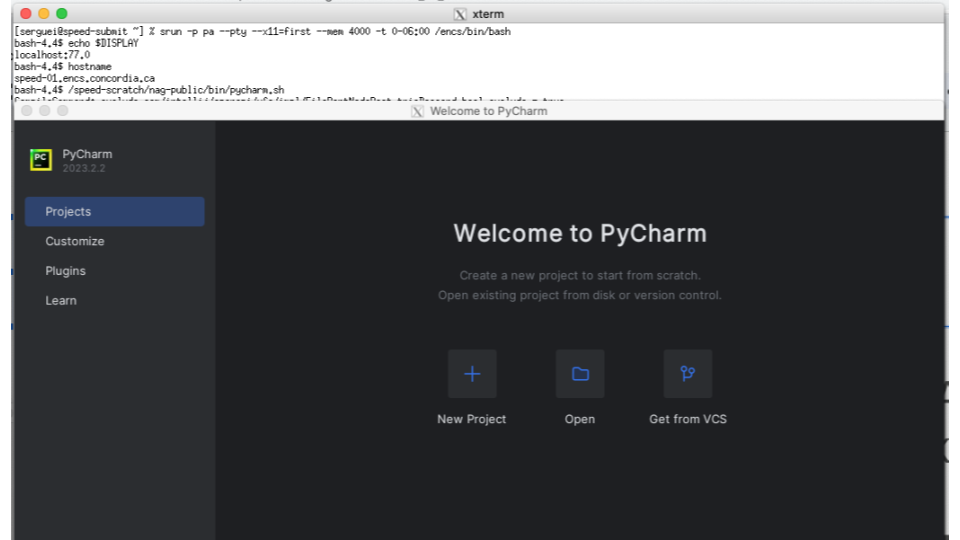
\includegraphics[width=\columnwidth]{images/pycharm}
		\caption{PyCharm Starting up on a Speed Node}
	\label{fig:pycharm}
\end{figure}

% ------------------------------------------------------------------------------
\subsubsection{Jupyter Notebooks}
\label{sect:jupyter}

This is an example of running Jupyter notebooks together with Singularity
(more on Singularity see \xs{sect:singularity-containers}).
Here we are using one of the OpenISS-derived containers (see \xs{sect:openiss-examples} as well).

\begin{enumerate}
\item
Use the \option{--x11} with \tool{salloc} or \tool{srun} as described in the above example

\item
Load Singularity module
\verb+module load singularity/3.10.4/default+

\item
Execute this Singularity command on a single line. It's best to save it in a shell script
that you could call, since it's long.
\scriptsize
\begin{verbatim}
srun singularity exec -B $PWD\:/speed-pwd,/speed-scratch/$USER\:/my-speed-scratch,/nettemp \
 --env SHELL=/bin/bash --nv /speed-scratch/nag-public/openiss-cuda-conda-jupyter.sif \
 /bin/bash -c '/opt/conda/bin/jupyter notebook --no-browser --notebook-dir=/speed-pwd \
 --ip="*" --port=8888 --allow-root'
\end{verbatim}
\normalsize

\item
Create an \tool{ssh} tunnel between your computer and the node (\texttt{speed-XX}) where Jupyter is
running (Using \texttt{speed-submit} as a ``jump server'') (Preferably: PuTTY, see \xf{fig:putty1} and \xf{fig:putty2})
\begin{verbatim}
ssh -L 8888:localhost:8888 speed-XX
\end{verbatim}
Don't close the tunnel.

\item
Open a browser, and copy your Jupyter's token, in the screenshot
example in \xf{fig:jupyter}; each time the token will be different,
as it printed to you in the terminal.

\small
\begin{verbatim}
http://localhost:8888/?token=5a52e6c0c7dfc111008a803e5303371ed0462d3d547ac3fb
\end{verbatim}
\normalsize

\item
Work with your notebook.

\end{enumerate}

\begin{figure}[htbp]
		\centering
		\fbox{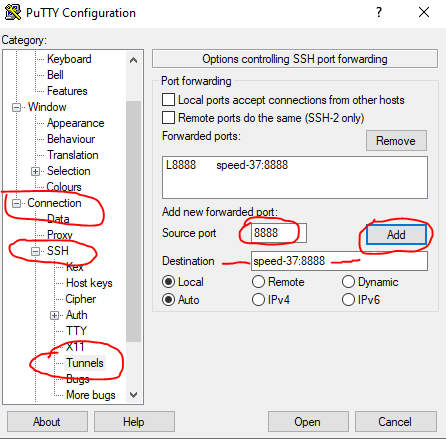
\includegraphics{images/putty1}}
	\caption{SSH tunnel configuration 1}
	\label{fig:putty1}
\end{figure}



\begin{figure}[htbp]
		\centering
		\fbox{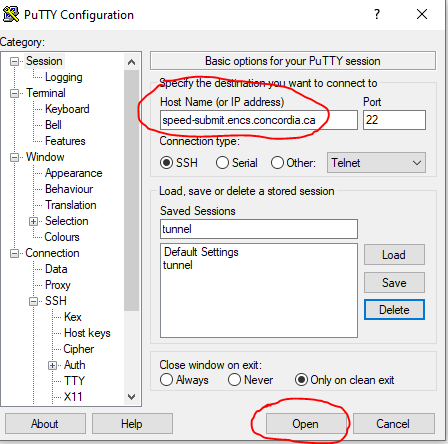
\includegraphics{images/putty2}}
	\caption{SSH tunnel configuration 2}
	\label{fig:putty2}
\end{figure}


\begin{figure}[htbp]
	\centering
	\fbox{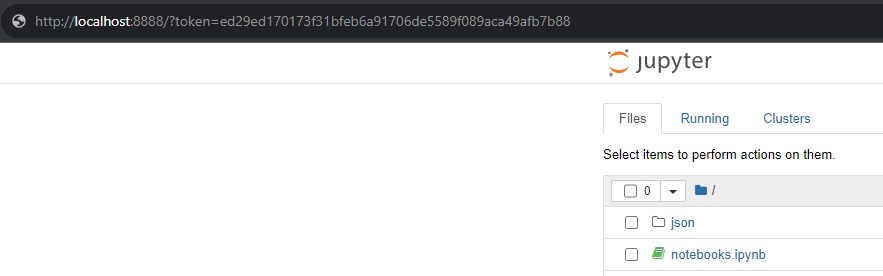
\includegraphics[width=1.00\textwidth]{images/jupyter.png}}
	\caption{Jupyter running on a Speed node}
	\label{fig:jupyter}
\end{figure}

% ------------------------------------------------------------------------------
\subsection{Scheduler Environment Variables}
\label{sect:env-vars}

The scheduler presents a number of environment variables that can be used in 
your jobs. You can invoke \tool{env} or \tool{printenv} in your
job to know what hose are (most begin with the prefix \texttt{SLURM}).
%
Some of the more useful ones are:
%\api{TMPDIR}, \api{SGE\_O\_WORKDIR}, and \api{NSLOTS}:

\begin{itemize}
\item
% TODO: verify temporal existence
\api{\$TMPDIR} -- the path to the job's temporary space on the node. It
\emph{only} exists for the duration of the job, so if data in the temporary space 
are important, they absolutely need to be accessed before the job terminates.

%\item
%\api{\$SGE\_O\_WORKDIR}=the path to the job's working directory (likely an
%NFS-mounted path). If, \texttt{-cwd}, was stipulated, that path is taken; if not, 
%the path defaults to your home directory.
\item
\api{\$SLURM\_SUBMIT\_DIR} -- the path to the job's working directory (likely an
NFS-mounted path). If, \option{--chdir}, was stipulated, that path is taken; if not, 
% TODO: verify if home or current:
the path defaults to your home directory.

% TODO: SLURM does not appear to have this
% SLURM_NTASKS
%\item
%\api{\$NSLOTS}=the number of cores requested for the job. This variable can 
%be used in place of hardcoded thread-request declarations. 

\item
\api{\$SLURM\_JOBID} -- your current jobs ID, useful for some manipulation
and reporting.

\item
\api{\$SLURM\_JOB\_NODELIST}=nodes participating in your job.

\item
\api{\$SLURM\_ARRAY\_TASK\_ID}=for array jobs (see \xs{sect:array-jobs}).

\item
See a more complete list here:

\small
\begin{itemize}
\item
\url{https://slurm.schedmd.com/srun.html#SECTION_INPUT-ENVIRONMENT-VARIABLES}
\item
\url{https://slurm.schedmd.com/srun.html#SECTION_OUTPUT-ENVIRONMENT-VARIABLES}
\end{itemize}
\normalsize

\end{itemize}

\noindent
In \xf{fig:tmpdir.sh} is a sample script, using some of these.

\begin{figure}[htpb]
    \lstinputlisting[language=csh,frame=single,basicstyle=\footnotesize\ttfamily]{tmpdir.sh}
    \caption{Source code for \file{tmpdir.sh}}
	\label{fig:tmpdir.sh}
\end{figure}

%

The final part of the job script involves the commands that will be executed by the job.
This section should include all necessary commands to set up and run the tasks
your script is designed to perform. You can use any Linux command in this section,
ranging from a simple executable call to a complex loop iterating through multiple commands.

\noindent \textbf{Best Practice}: prefix any compute-heavy step with \tool{srun}.
This ensures you gain proper insights on the execution of your job.

\noindent Each software program may have its own execution framework, as it's the script's author (e.g., you)
responsibility to review the software's documentation to understand its requirements.
Your script should be written to clearly specify the location of input and output files and the degree of parallelism needed.

\noindent Jobs that involve multiple interactions with data input and output files, should make use of \api{TMPDIR},
a scheduler-provided workspace nearly 1~TB in size.
\api{TMPDIR} is created on the local disk of the compute node at the start of a job, offering faster I/O operations
compared to shared storage (provided over NFS).

%TO BE DELETED 
% example in /home/n/nul-uge/templateTMPDIR.sh is not accessible.

%An sample job script using \api{TMPDIR} is available at \texttt{/home/n/nul-uge/templateTMPDIR.sh}: 
%the job is instructed to change to \api{\$TMPDIR}, to make the new directory \texttt{input}, to copy data from
%\texttt{\$SLURM\_SUBMIT\_DIR/references/} to \texttt{input/} (\api{\$SLURM\_SUBMIT\_DIR} represents the
%current working directory), to make the new directory \texttt{results}, to
%execute the program (which takes input from \texttt{\$TMPDIR/input/} and writes
%output to \texttt{\$TMPDIR/results/}), and finally to copy the total end results
%to an existing directory, \texttt{processed}, that is located in the current
%working directory.
% TODO: verify:
%\api{TMPDIR} only exists for the duration of the job, though,
%so it is very important to copy relevant results from it at job's end.